\icode{E-MCH-MU-L3-261026-001}
（多选）
如图所示，\(a\)、\(b\)两小球分别从半圆轨道顶端和斜面顶端以大小相等的初速度\(v_0\)同时水平抛出。已知半圆轨道的半径\(R\)与斜面竖直高度相等，斜面底边长是其竖直高度的2倍。若小球\(a\)能落到半圆轨道上，小球\(b\)能落到斜面上，\(a\)、\(b\)均可视为质点，重力加速度为\(g\)，则\paren[]

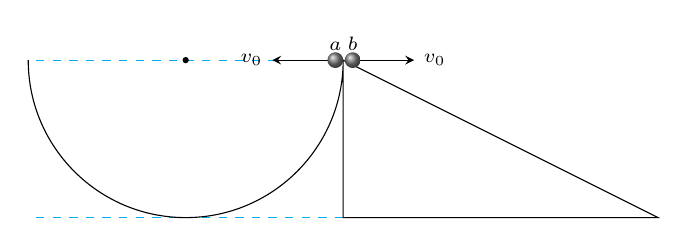
\begin{tikzpicture}[>=stealth,font=\scriptsize]
	\draw[dashed,cyan] (0,2)--(-4,2) (0,0)--(-4,0);
	\fill (-2,2) circle(.04);
	\draw (0,2) arc(0:-180:2) (0,2)--(0,0)--(4,0)--cycle;
	\draw[->] (-.1,2)--++(-.8,0)node[left]{ \(v_0\)};
	\draw[->] (0.1,2)--++(.8,0)node[right]{ \(v_0\)};
	\foreach \c/\t in {(-.1,2)/a,(.12,2)/b}
		\shade[ball color=gray] \c node[above]{ \(\t\)} circle(.1);
\end{tikzpicture}
\begin{choices}
	\item 如果\(a\)球落在半圆轨道最低点，则其速度方向竖直向下
	\item \(b\)球落在斜面上时，其速度方向与水平面夹角的正切值为0.5
	\item \(a\)、\(b\)两球如果同时落在半圆轨道和斜面上，则其初速度\(v_0 = 2\sqrt{\frac{2gR}{5}}\)
	\item 无论\(a\)球初速度\(v_0\)多大，\(a\)球均不可能垂直落在半圆轨道上
\end{choices}
\begin{answer}
	CD\qquad 提示：
\end{answer}